%%%%%%%%%%%%%%%%%%%%%%%%%%%%%%%%%%%%%%%%%%%%%%%%%%%%%%%%%%%%%%%%%%%%%%%%
%%%  THIS TEX FILE IS TO GENERATE PDF FILE FOR 
%%% 
%%%  COPYRIGHT (C) JIMMY LIN, 2013, UT AUSTIN
%%%%%%%%%%%%%%%%%%%%%%%%%%%%%%%%%%%%%%%%%%%%%%%%%%%%%%%%%%%%%%%%%%%%%%%%
\documentclass[11pt,a4paper]{article}
%%%%%%%%%%%%%%%%%%%%%%%%%%%%%%%%%%%%%%%%%%%%%%%%%%%%%%%%%%%%%%%%%%%%%%%%
%%%  PACKAGES USED IN THIS TEX SOURCE FILE
%%%%%%%%%%%%%%%%%%%%%%%%%%%%%%%%%%%%%%%%%%%%%%%%%%%%%%%%%%%%%%%%%%%%%%%%
\usepackage{geometry,amsthm,amsmath,graphicx,fancyheadings,fancybox}
\usepackage{tikz}
\usepackage[colorlinks,
            linkcolor=blue,
            anchorcolor=red,
            citecolor=green
            ]{hyperref}
\usepackage{/Users/JimmyLin/workspace/latexTemplate/UTA_CS/JS}
\usepackage{/Users/JimmyLin/workspace/latexTemplate/UTA_CS/JSASGN}
%%%%%%%%%%%%%%%%%%%%%%%%%%%%%%%%%%%%%%%%%%%%%%%%%%%%%%%%%%%%%%%%%%%%%%%%
%%% MACROS CONTAINING THE FILE INFORMATION
%%%%%%%%%%%%%%%%%%%%%%%%%%%%%%%%%%%%%%%%%%%%%%%%%%%%%%%%%%%%%%%%%%%%%%%%
\renewcommand{\COURSE}{CS331 Algorithm}
\renewcommand{\LECTURER}{Greg Plexton}
\renewcommand{\TUTOR}{Chunzhi Zhu}
\renewcommand{\TASK}{Assignment 04}
\renewcommand{\RELEASEDATE}{March. 09 2014}
\renewcommand{\DUEDATE}{March. 24 2014}
\renewcommand{\TIMECONSUME}{10 hours}
%%%%%%%%%%%%%%%%%%%%%%%%%%%%%%%%%%%%%%%%%%%%%%%%%%%%%%%%%%%%%%%%%%%%%%%%
%%% DOCUMENTATION STARTS FROM HERE 
%%%%%%%%%%%%%%%%%%%%%%%%%%%%%%%%%%%%%%%%%%%%%%%%%%%%%%%%%%%%%%%%%%%%%%%%
\begin{document}
%%%%%%%%%%%%%%%%%%%%%%%%%%%%%%%%%%%%%%%%%%%%%%%%%%%%%%%%%%%%%%%%%%%%%%%%
%% TITLE PAGE
%%%%%%%%%%%%%%%%%%%%%%%%%%%%%%%%%%%%%%%%%%%%%%%%%%%%%%%%%%%%%%%%%%%%%%%%
\begin{titlepage}
    \maketitle
\end{titlepage}
%%%%%%%%%%%%%%%%%%%%%%%%%%%%%%%%%%%%%%%%%%%%%%%%%%%%%%%%%%%%%%%%%%%%%%%%
%% CONTENT PAGE: TABLEOFCONTENTS, LISTOFTABLES, LIST OF FIGURES
%%%%%%%%%%%%%%%%%%%%%%%%%%%%%%%%%%%%%%%%%%%%%%%%%%%%%%%%%%%%%%%%%%%%%%%%
\renewcommand{\contentsname}{Contents}
\begin{center} 
    \tableofcontents 
\end{center}
\newpage
%%%%%%%%%%%%%%%%%%%%%%%%%%%%%%%%%%%%%%%%%%%%%%%%%%%%%%%%%%%%%%%%%%%%%%%%
%%% GENERAL DOCUMENTATION BEGINS 
%%%%%%%%%%%%%%%%%%%%%%%%%%%%%%%%%%%%%%%%%%%%%%%%%%%%%%%%%%%%%%%%%%%%%%%%
\newcommand{\wm}[1]{\ensuremath{w(M_{#1})}}
\newcommand{\wmp}[1]{\ensuremath{w(M'_{#1})}}
\newcommand{\wmi}{\ensuremath{w(M_i)}}
\newcommand{\wmip}{\ensuremath{w(M'_i)}}
\newcommand{\constantTime}{\ensuremath{\mathcal{O}(1)}}
\newcommand{\linearTime}{\ensuremath{\mathcal{O}(n)}}
\newcommand{\lbw}[1]{\ensuremath{a_{#1} q_{#1} + b_{#1}}}  %% linear bid weight
\newcommand{\sbw}[1]{\ensuremath{m_{#1}}}
\section{Exercise 1}
\ovalbox{
\begin{minipage}{15cm}
\textbf{Exercise 1.} Let $G = (U, V, E)$ be a configuration. Prove that if $p$ is
a stable price vector for $G$ and $v$ is an item in $V$,then $p_v$ is at least
the start price of $v$.
\end{minipage} } \\[0.5cm]

\begin{proof} [Overview]
We provide the proof by contradiction. We first assume that there exist a item $v$
for which, the $p_v$ can be less than the start price of item $v$. That is,
\begin{align} \label{tocontra}
    \exists v \in V,  p_v < p^*_v 
\end{align}
where $p^*_v$ is the start price of item
$v$. And there are two cases we should consider as follows:
\begin{itemize}
    \item{for item $v$, there is no unit-demand bid wins it}
    \item{for item $v$, there is at least one unit-demand bid wins it}
\end{itemize}
We provide dicussion over two cases above, and then show the contradiction in
each case.
\end{proof}

\noindent
    Notational explanation:
\begin{itemize}
    \item{$p_{v}^{R}$ is the reserve price for item $v$}
    \item{$p_{v}^{*}$ is the start price for item $v$}
    \item{$w(u,v)$ is the unit-demand bid $u$ 's bidding price to item $v$}
\end{itemize}

\begin{proof}[No unit-demand bid wins it]
    Since unit-demand bid $u$ does not win item $v$, we have 
    $ w(u,v) \leq p_{v}^{R}$
    There are two subcases when if there is no unit-demand bid wins it. 
    \begin{itemize}
        \item{$\neg \exists (u,v),\ w(u,v) \geq p_{v}^{R}$, in this case, the
                $p_v = p_{v}^{*}$, contradicts to \eqref{tocontra}}   
        \item{$\exists (u,v),\ w(u,v) \geq p_{v}^{R}$, $p_v = max(w(u,v),
                w(u',v'), ..) \geq p_{v}^{*}$, contradicts to \eqref{tocontra}}
    \end{itemize}
\end{proof}

\begin{proof}[At least one unit-demand bid wins it]
    Only consider the first unit-demand bid $u$ winning item $v$. Since $u$
    wins the item $v$, we have 
    \begin{align}
        w(u,v) \geq p_{v}^{R} \geq p_{v}^{*}
    \end{align}
    At this moment, the $p_{v} = p_{v}^{R} \geq p_{v}^{*}$. And the later
    unit-demand bid $u'$ which wins item $v$ must satisfy
    \begin{align}
        w(u',v) \geq w(u,v) 
    \end{align}
    And at that time, the $p_v$ in price vector will be updated to be
    $w(u,v)$, which is larger than previous price. Hence, we can conclude that 
    \begin{align}
        p_v \geq p_{v}^{*}
        \end{align}
    This contradicts to \eqref{tocontra}.
    An formal alternative to prove this is to have induction on the number of
    unit-demand bid ever winning item $v$ and show a persistent contradiction.
    But here we just provide brief proof. 
\end{proof}
\noindent
Since in all possibilities indicates a contradiction to \eqref{tocontra}, we
can negate the initial assumption to have
\begin{align} \label{tonegate}
    \neg \exists v \in V,  p_v < p^*_v 
\end{align}
That is to conclude, 
\begin{align} \label{tonegate}
    \forall v \in V,  p_v \geq p^*_v 
\end{align}

\newpage
\section{Exercise 2}
\ovalbox{
\begin{minipage}{15cm} 
    \textbf{Exercise 2.} Let $G = (U, V, E)$ be a configuration, let
    $(M, p)$ and $(M', p)$ be stable solutions for $G$, let $(u,v)$ be an edge
    in $M$, and assume that $w(u,v) > p_v$. Prove that $u$ is matched to some item
    $v'$ in $M'$, and $w(u,v) - p_v = w(u,v') - p_v'$.
\end{minipage} } \\

    Since $(M, p)$ is stable solution, and $(u,v) \in M$, we can instantiate
    the second property of stable solution and have
    \begin{align}
        w(u,v) - p_v \geq w(u,v') - p_{v'}
    \end{align}

    Since we assume that $w(u,v) > p_v$, it can be avoided that two bids have
    the same bidding highest price for item $v$ ($p_v$ is the second highest
    bidding price). Hence, the other MWMCM is not
    made by the instability as the same highest bidding price.

    Similarly for stable solution $(M', p)$, we have
    \begin{align}
        w(u,v') - p_{v'} \geq w(u,v) - p_{v}
    \end{align}

    Therefore, we have
    \begin{align}
        w(u,v) - p_v = w(u,v') - p_{v'}
    \end{align}

\newpage
\section{Exercise 3}
\ovalbox{
\begin{minipage}{15cm} 
    \textbf{Exercise 3.} Let $G = (U, V, E)$ be a configuration. Prove that if
    $(M, p)$ is a stable solution for $G$, then $M$ is an MWMCM of $G$. Hint:
    Let $M′$ be an MWMCM of $G$, and make use of the fact that the bipartite
    graph $G′ = (U,V,M \oplus M′)$ consists of a collection of disjoint paths and
    cycles, where each path and cycle in the collection is of even length.
\end{minipage} }

\begin{proof}[Overview]
    Let $M'$ be an MWMCM of $G$, and it is easy to see the fact that the bipartite graph
    $G$ = $(U,V,M)$ consists of a collection of disjoint paths and cycles,
    where each path and cycle in the collection is of even length. Hence,
    there are {\bf three cases} we need to consider for $G'$, {\bf (1) cycle (2) path with
    unit-demand bid as endpoint (3) path with item as endpoint}. The intuitive
    idea of our proof is that in all cases mentioned above, the total weight
    of edges in stable solution $M$ is no less than the total weight of edges
    in the MWMCM $M'$ and since $M'$ is MWMCM (total weight should be no less
    than any MCM), the only possible scenario is that $M$ is also a MWMCM. 

\end{proof}

Before diving into the detailed proof for all three cases, we first
domonstrate you the representative graph for convenient comprehension.

% drawing
%{{{
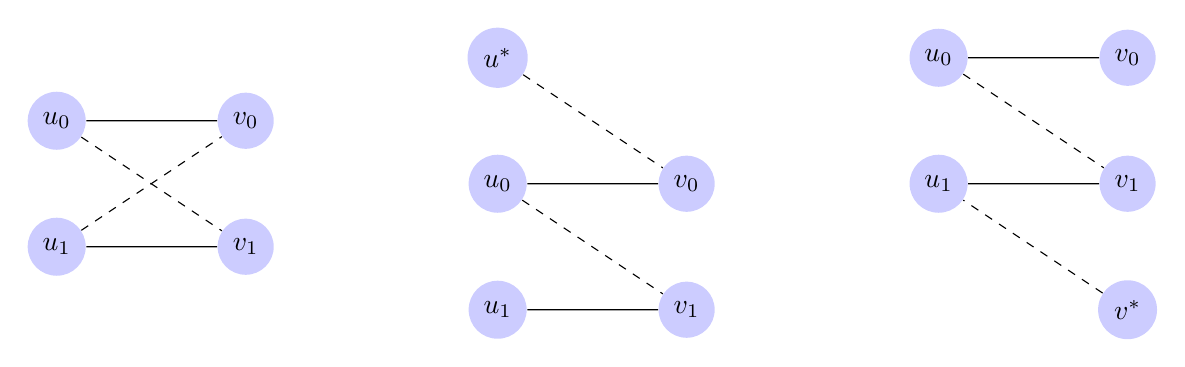
\begin{tikzpicture}
  [scale=.8,auto=left,every node/.style={circle,fill=blue!20}]
  \node (u0) at (3, 8) {$u_0$};
  \node (u1) at (3, 6)  {$u_1$};
  \node (v0) at (6, 8) {$v_0$};
  \node (v1) at (6, 6)  {$v_1$};

  \node (us) at (10, 9) {$u^*$};
  \node (u00) at (10, 7) {$u_0$};
  \node (u11) at (10, 5)  {$u_1$};
  \node (v00) at (13, 7) {$v_0$};
  \node (v11) at (13, 5)  {$v_1$};

  \node (u000) at (17, 9) {$u_0$};
  \node (u111) at (17, 7)  {$u_1$};
  \node (v000) at (20, 9) {$v_0$};
  \node (v111) at (20, 7)  {$v_1$};
  \node (vs) at (20, 5) {$v^*$};

  \foreach \from/\to in {u0/v0,u1/v1}
    \draw  (\from) -- (\to);
  \foreach \from/\to in {u0/v1,u1/v0}
    \draw [dashed] (\from) -- (\to);

  \foreach \from/\to in {u00/v00,u11/v11}
    \draw (\from) -- (\to);
  \foreach \from/\to in {u00/v11,us/v00}
  \draw [dashed] (\from) -- (\to);

    \foreach \from/\to in {u000/v000,u111/v111}
    \draw (\from) -- (\to);
  \foreach \from/\to in {u000/v111,vs/u111}
  \draw [dashed] (\from) -- (\to);
\end{tikzpicture}
%}}}

Note that the case shown above from left to right are (1), (2) and (3)
respectively. And for every edge shown above, if it is full line, then it is
in the stable solution MCM $M$, while the dashed line represents pairs in
MWMCM $M'$.

Next, we are going to provide proof for three general cases. For specific
notation reference, you can refer to the representative graph.

\begin{proof}[Cycle]

    The proof is simple in this case. Since every bid node is in a cycle, we
    have that in $G'$, each bid node has at most two edges connecting to it,
    one is in $M$ and the other in $M'$. The same property also applies to the
    item node. Otherwise, it cannot form a cycle.
    According to the second property of stable solution, we have 

    \begin{align}
        \forall u, (u,v) \in M,\ (u, v') \in M', s.t.\  w(u, v) - p_v \geq w(u, v') - p_{v'}
    \end{align}

    Sum up all inequalities, and then we will have all item price removed on
    both side of the resulted inequality, 

    \begin{align} \label{cycle:seconproperty}
        \sum_{u} ( w(u, v) - p_v) & \geq \sum_{u} ( w(u, v') - p_{v'} ) 
    \end{align}
    
    In one cycle, it can be easily observed that 

    \begin{align} \label{cycle:observation}
        \sum_{u} p_v & = \sum_{u}  p_{v'}
    \end{align}

    Note that in one cycle, the set of bid nodes can only be matched to the
    same set of item nodes, regardless of the MCM we talks about. By \eqref{cycle:seconproperty}
    and \eqref{cycle:observation}, we have

    \begin{align}
        \sum_{u} w(u, v) & \geq \sum_{u}  w(u, v')
    \end{align}

    Thus, in one cycle subgraph, the total weight of edges in $M$ is no less
    than the total weight of edges in $M'$.

\end{proof}

\begin{proof}[Unit-demand bid as endpoint]

    In case of a path with unit-demand bid as its endpoint, things are a
    little more complicated. Since $u^{*}$ is unmatched in stable solution
    MCM $M$ and according to the third property of stable solution , we have
    
    \begin{align} 
        \forall v,\ w(u^{*}, v) \leq p_{v}
    \end{align}

    Instantiate it, we have 
    \begin{align}  \label{unit:v1}
         - w(u^{*}, v_1) \geq - p_{v_1} 
    \end{align}

    For every immediate unit-demand bid $u$, it is easy to see that they all
    have one edge in $M$ and one in $M'$. In terms of the second property of
    stable solution, 

    \begin{align} \label{Unit:foreach}
        \forall u',\ degree(u') = 2,\ (u', v') \in M,\ (u', v'') \in M',\
        s.t.\  \\
        w(u',v') - p_{v'} \geq w(u', v'') - p_{v''}
    \end{align}

    For the other end edge $(u_{n}, v_{n})$ of this path, we can have 

    \begin{align} 
        p_{v_{n}} &\leq w(u_{n}, v_{n}) \\
        - p_{v_{n}} &\geq - w(u_{n}, v_{n})  \label{unit:vn}
    \end{align}

    Sum up \eqref{Unit:foreach}, we have

    \begin{align}
        \sum_{u'} (w(u',v') - p_{v'}) & \geq \sum_{u'} (w(u', v'') - p_{v''}) \\
        \sum_{u'} (w(u',v')) - p_{v_1} & \geq 
        \sum_{u'} (w(u', v'')) - p_{v_{n}}   \label{unit:origin}
    \end{align}

    According to the \eqref{unit:v1}, we have 

    \begin{align} \label{unit:derive1}
       \sum_{u'} (w(u',v')) - w(u^{*}, v_1) \geq \sum_{u'} (w(u',v')) - p_{v_1} 
    \end{align}

    According to the \eqref{unit:vn}, we have 

    \begin{align} \label{unit:derive2}
        \sum_{u'} (w(u', v'')) - p_{v_{n}} \geq \sum_{u'} (w(u', v'')) -
        w(u_{n}, v_{n})
    \end{align}

    Based on \eqref{unit:origin}, \eqref{unit:derive1} and
    \eqref{unit:derive2}, we have

    \begin{align}
        \sum_{u'} (w(u',v')) - w(u^{*}, v_1) \geq \sum_{u'} (w(u', v'')) -
        w(u_{n}, v_{n}) \\
        \sum_{u'} (w(u',v')) +  w(u_{n}, v_{n}) \geq \sum_{u'} (w(u', v'')) +
         w(u^{*}, v_1)
    \end{align}

    Since $(u_n, v_n)$ is in stable solution MCM $M$, and $(u^{*}, v_1)$ is in
    MWMCM $M'$, we can conclude that in one path with unit-demand bid as
    endpoint, the total weight of edges in $M$ is no less than the total
    weight of edges in $M'$

\end{proof}

\begin{proof}[Item as endpoint]

    This case is more complicated than previous one. Since if one item is not matched by
    any unit-demand bid, it will be matched by dummy bid, say reserve bid. 

    Similarly to previous, in graph $G'$, the unit-demand bid has the
    following property.

    \begin{align}
        \forall u',\ degree(u') = 2,\ (u', v') \in M,\ (u', v'') \in M',\
        s.t.\ \nonumber \\
        w(u',v') - p_{v'} \geq w(u', v'') - p_{v''} \label{Item:foreach}
    \end{align}

    Sum up all inequalities, we have 
    \begin{align}
        \sum_{u'}  (w(u',v')) - p_{v_0} &\geq \sum_{u'}  (w(u',v'')) -
        p_{v^{*}} \\
        \sum_{u'}  (w(u',v')) +  p_{v^{*}} &\geq \sum_{u'}  (w(u',v'')) +  p_{v_0} 
    \end{align}

    Since the $p_{v_0}$ is the reserve price of item $v_0$, which is counted
    in MWMCM, and $p_{v^{*}}$ is the start price of item $v^{*}$, which is
    counted in stable solution, it can be concluded that the total weight of
    edges in $M$ is no less than the total weight of edges in $M'$.

\end{proof}


\begin{proof}[Epilogue]
    Since $G'$ consists of a collection of cycles
    and path, and we have proven that the total weight of edges
    in $M$ is no less than the total weight of edges in $M'$ for all cases, we
    can conclude that

    \begin{align}
        w (M) \geq w (M')
    \end{align}

    Since $M'$ is MWMCM, we have
    \begin{align}
        w (M) \leq w (M')
    \end{align}

    Hence, the only possibility can be
    \begin{align}
        w (M) = w (M')
    \end{align}

    Therefore, the MCM in stable solution $(M,p)$ is also MWMCM.
\end{proof}

\newpage
\section{Exercise 4}
\ovalbox{
\begin{minipage}{15cm} 
    \textbf{Exercise 4.} Let $G$ be a configuration, let $M$ be an MWMCM of
    $G$, and let $p$ be a price vector for $G$. Prove that digraph $(G,M,p)$
    does not contain a directed cycle of positive weight.
\end{minipage} }

\begin{proof} [Proof by Contradiction]
    Let us assume that $digraph(G,M,p)$ does contain a directed cycle of
    positive weight. Since in the cycle C, all nodes are matched in $G$, we
    only need to refer to the first and second rule of provided $G'$
    formation.
    And here we represent the cycle C which has positive weight,
    by indexing involved bid set ${u_0, .., u_n}$, and item set ${v_0, .., v_n}$,
    such that

    $$ \forall i \in [0,n], (u_i, v_i) \in M $$

    According to the edge formation of $E'$ of $G'(V', E')$, in cycle C, each
    node must have degree of size 2, one incoming edge and one outgoing edge.
    For each item node indexed by $i$, the outgoing edges can be explained
    mathematically as follows,

    \begin{align} \label{e4_eachItem}
        (u_i, v_i) \in M  
    \end{align}

    For each bid node indexed by $i$, whose outgoing edge is $(u_i, v_j)$ ($j
    \neq j$), we
    can treat it as 

    \begin{align} \label{e4_eachBidNode}
        w(u_i, v_i) - p_{v_i} \leq w(u_i, v_j) - p_{v_j}
    \end{align}

    Since all the corresponding edges in \eqref{e4_eachItem} on $E'$ has
    weight 0, there must be {\bf at least one inequality in \eqref{e4_eachBidNode}
    having non-equal relationship. Otherwise, the cycle C does have positive
    weight. }
    
    By summing up all inequalities in \eqref{e4_eachBidNode} and cancel out
    all terms about certain component of price vector, we have
    \begin{align}
        \sum_i \big( w(u_i, v_i) \big) < 
            \sum_i \big( w(u_i, v_j) \big)
    \end{align}

    The derived inequality indicates that for each $u_i$, the matching $(u_i,
    v_j) \in M$ rather than $(u_i, v_j)$.
    Apparently, this contradicts to our encoding scheme of MWMCM $M$ at the very
    beginning.

    Thus, there does no exist a cycle of positive weight in digraph $(G,M,p)$
\end{proof}

%%%%%%%%%%%%%%%%%%%%%%%%%%%%%%%%%%%%%%%%%%%%%%%%%%%%%%%%%%%%%%%%%%%%%%%%
%%% General Documentation ends
%%%%%%%%%%%%%%%%%%%%%%%%%%%%%%%%%%%%%%%%%%%%%%%%%%%%%%%%%%%%%%%%%%%%%%%%
\end{document}
